%% -*- eval: (flyspell-mode 1); -*-

\chapter{Extraction et formalisation du parallélisme}

Le parallélisme dans un programme informatique est difficile à trouver automatiquement et la plupart du temps il est exprimé explicitement par le développeur. Il est alors nécessaire de lui offrir des outils permettant d'écrire le code parallèle simplement, en lui proposant notamment des fonctions et des mots-clés dans le langage choisi qui sont en accord à la fois avec les besoins matériels et avec les besoins algorithmiques. Ce chapitre dresse d'abord un état de l'art des principales solutions existantes ainsi que des précisions sur le matériel qu'elles exploitent, puis introduit les principaux objectifs du DSEL développé pendant le stage.

\section{Contexte}

Les applications parallèles sont utilisées depuis un certain nombre d'années afin d'obtenir des performances (en matière de rapidité, et en matière de taille du problème traité), or il est difficile d'écrire des codes parallèles. À ce titre divers outils pour faciliter la parallélisation sont apparus, tels que \textsf{ParaScope} dès $1989$ \cite{Art24} qui est éditeur interactif de code parallèle. Ces outils se décomposent en de nombreuses catégories selon les utilisateurs qu'ils visent, et selon le parallélisme qu'ils permettent. Une partie d'entre elles sont détaillées dans les paragraphes suivants. En second lieu sont introduits les stencils, qui constituent la classe de problèmes étudiée pendant ce stage. Enfin la hiérarchie de la mémoire du matériel est rappelée afin de mieux comprendre les problématiques liées aux stencils.

\subsection{Expression du parallélisme}
\label{sec:biblio}

Décrire les problèmes à résoudre et le parallélisme qu'ils peuvent utiliser peut se faire de différentes manières avec les moyens actuels. Notamment il est possible d'identifier cinq catégories que sont : les langages de haut niveau dédiés à un domaine scientifique (dont les acteurs ne sont pas informaticiens), les langages et compilateurs pour les développeurs de métier (mais non obligatoirement spécialistes du HPC), l'ensemble des bibliothèques ou DSEL et supports d'exécution dédiés à la parallélisation (destinés aux spécialistes du HPC), les outils de formalisation des algorithmes employés (destinés aux spécialistes du HPC) et enfin les bibliothèques ou DSEL dédiés à un problème scientifique (et masquant la parallélisation, donc pour des scientifiques/développeurs non spécialistes du HPC).

\paragraph{Langages de haut niveau dédiés à un domaine scientifique.}
Les langages dédiés aux scientifiques sont la plupart du temps des outils de simulation à destination d'experts dans ce domaine. Dans le cas des mathématiques par exemple, de nombreux logiciels définissant leur propre langage existent : \textsf{\href{http://www.wolfram.com/mathematica/}{Mathematica}}, \textsf{\href{http://fr.mathworks.com/}{MATLAB}} ou encore \textsf{\href{http://pari.math.u-bordeaux.fr/}{PARI/GP}} ; et une partie de leurs algorithmes sont parallélisés (au moins au niveau d'un processeur) pour des raisons de performances. Des initiatives sont également présentes dans la physique comme \textsf{QIRAL} \cite{Art13,Art14} pour la chromodynamique quantique. À partir d'algorithmes décrits en \LaTeX, \textsf{QIRAL} permet de générer un code parallèle optimisé pour les processeurs des ordinateurs courants --- mais pas pour les supercalculateurs ---, il s'appuie pour cela sur le système de réécriture \textsf{Maude} \cite{Art12}. La logique pour tous ces langages est alors la suivante : offrir à l'utilisateur les mêmes fonctions qui sont connues dans son domaine, en cachant l'implantation et la parallélisation de ces fonctions (telles qu'un calcul de facteurs premiers par exemple).

\paragraph{Langages dédiés au parallélisme.}
Quant il s'agit de développeurs souhaitant écrire du code parallèle sans forcément dépendre des subtilités des machines d'exécutions, différents langages spécifiques ont été créés. De manière générale, il s'agit en fait d'un langage déjà connu (\textsf{Java} ou \textsf{C/C++}) auquel sont ajoutés quelques mots-clés ou éléments de syntaxes (souvent pour les tableaux notamment) ; \textsf{\href{http://chapel.cray.com/}{Chapel}}, \textsf{\href{https://www.cilkplus.org/}{Cilk}}, \textsf{\href{http://upc.lbl.gov/}{UPC}}, \textsf{Lime} \cite{Art8}, \textsf{\href{http://x10-lang.org/}{X10}} et le langage proposé dans l'article \cite{Art10} rentrent dans cette catégorie. Alors que les trois premiers cités sont très proches des langages d'origine, les trois derniers sont plus éloignés et proposent des paradigmes différents (comme les Map/Reduce dans \textsf{Lime} ou les horloges dans \textsf{X10}). Avec ces langages viennent souvent les compilateurs associés, toutefois parfois il s'agit plus simplement de réécriture automatique de code (vers un langage déjà existant) comme proposé par \textsf{Par4All} \cite{Ths2}. \textsf{Par4All} peut d'ailleurs être considéré comme un éditeur de code dédié au parallélisme, de même que le projet \textsf{Eclipse \href{http://www.eclipse.org/ptp/}{PTP}} (Parallel Tools Platform) ou les projets présentés dans les articles \cite{Art23,Art25}. Ces éditeurs rassemblent alors généralement plusieurs outils, et sont plus interactifs, mais leur parallélisation n'est pas toujours optimale.

\paragraph{Bibliothèques, DSEL et supports d'exécutions pour l'expression du parallélisme.}
Pour atteindre un parallélisme optimal, il est souvent nécessaire de descendre à un niveau plus proche du matériel. Plutôt que d'introduire quelques mots-clés supplémentaires, il s'agit alors de plusieurs dizaines de fonctions regroupées dans des bibliothèques. Il faut alors parfois utiliser différentes bibliothèques afin de gérer les différents niveaux de parallélisme (notamment interprocesseur et intraprocesseur). La bibliothèque utilisée dans le cadre du stage en fait partie : \textsf{\href{https://www.khronos.org/sycl}{SYCL}}. C'est la bibliothèque qui est du plus haut niveau tout en offrant le plus de possibilités. La bibliothèque connue qui s'en rapproche le plus est \textsf{\href{https://www.khronos.org/opencl/}{OpenCL}} mais nécessite déjà plus d'efforts notamment pour gérer les communications entre les processeurs. En revanche, \textsf{\href{http://openmp.org/wp/}{OpenMP}} (qui est intégrée dans la plupart des compilateurs pour \textsf{Fortran}, \textsf{C/C++}) est beaucoup plus simple mais ne s'utilise que pour les processeurs génériques et non les processeurs graphiques. D'autres bibliothèques sont justement dédiées à la gestion de plusieurs types de processeurs en même temps, il s'agit des \emph{supports d'exécutions} tels que \textsf{\href{http://starpu.gforge.inria.fr/}{StarPU}} ou \textsf{\href{http://icl.utk.edu/parsec/}{PaRSEC}}. Comme la plupart des problèmes parallélisés sont liés à l'utilisation de grands tableaux, \textsf{Kokkos} \cite{Web5} et \textsf{\href{http://hpc.pnl.gov/globalarrays/}{Global Arrays}} permettent de simplifier leur utilisation et répartition sur les différents processeurs, mais ils ne gèrent pas le lancement des calculs contrairement aux supports d'exécutions. Plus spécifiquement encore l'article \cite{Art2} propose une solution simplifiant l'utilisation des tableaux avec le parallélisme, au sein d'un processeur. 


\paragraph{Formalisation des algorithmes.}
La formalisation des algorithmes parallèles se fait à travers différents outils comme la représentation polyédrique, utilisée lorsqu'il s'agit de parcours de tableaux au sein de boucles affines. Cette représentation permet d'ailleurs de mieux classifier les algorithmes, notamment en squelettes comme dans \textsf{SkePU} et \textsf{Bones} \cite{Art4,Art3,Art9}. Ces squelettes permettent de définir le motif d'accès aux données des tableaux impliqués dans le calcul de façon précise et ainsi de l'optimiser. Un tel exemple de motif --- plutôt général --- est le paradigme de \emph{Map/Reduce} qui est proposé par \textsf{SkePU} \cite{MstThs1} (ainsi que par le langage dédié \textsf{Lime} cité plus-haut). Cependant tous les algorithmes ne décrivent pas un calcul : certains sont au contraire destinés à ordonnancer les calculs, c'est-à-dire les répartir sur les différents processeurs disponibles. Encore plutôt à l'état de concept, c'est dans ce but que sont utilisés les \emph{composants} permettant les prédictions (et optimisations) du temps d'exécution tels que dans l'article \cite{Art7}, où les algorithmes sont associés à des informations concernant leur coût. Par ailleurs dans \textsf{SkePU} \cite[p.~78]{Ths1} les \emph{smart containers} (ou \emph{conteneurs intelligents}) aident la gestion des communications avec la mémoire (et aussi les prédictions de temps) en forçant l'utilisateur à informer la bibliothèque de la mémoire qu'il utilise. La formalisation des algorithmes se fait donc généralement par squelette ou composants en ce qui concerne les calculs à effectuer, et conteneurs en ce qui concerne les données à utiliser.

\paragraph{Bibliothèques et DSEL dédiés à un domaine scientifique.}
Certaines bibliothèques sont destinées à des domaines d'application particuliers et cachent le parallélisme qu'elles utilisent. Par exemple il peut s'agir des \textsf{BLAS} pour les opérations d'algèbre linéaire simple, et de \textsf{\href{http://www.netlib.org/lapack/}{LAPACK}} pour les opérations plus complexes (de décomposition en valeurs propres par exemple). \textsf{\href{http://www.fftw.org/}{FFTW}} est quant à elle dédiée aux transformées de Fourier, et \textsf{\href{http://sourceforge.net/projects/blitz/}{Blitz++}} dédiées aux calculs sur les vecteurs. Toutefois \textsf{Blitz++} est assez vieux (une quinzaine d'années) et n'utilise donc pas toutes les possibilités offertes par les langages modernes (au moins pour la version en \textsf{C++}).


\subsection{Cas d'application: les stencils}
\label{sec:stencil_base}

De nombreux problèmes notamment physiques ou mathématiques sont simulés sur ordinateur et sont alors discrétisés. Ils emploient alors souvent des calculs sur des grilles d'éléments qui sont regroupés sous le nom de \emph{stencils}. Dans ces problèmes chaque élément au sein d'une grille est calculé en fonction des valeurs de ses voisins. En une dimension, il s'agirait par exemple d'un tableau dans lequel chaque élément reçoit la somme de son voisin de droite et de celui de gauche. Compte-tenu de l'utilisation très répandue des stencils\footnote{Elle dépasse même le cadre scientifique car les stencils sont également utilisées par exemple dans le calcul des graphismes de jeux vidéos \cite{Art15}. Dans les deux cas la rapidité des calculs est un des objectifs principaux, à tel point que la précision des résultats est volontairement atténuée dans l'article précédent.}, leur parallélisation est primordiale afin d'accélérer ces calculs. Divers outils dédiés ont donc été créés : des bibliothèques de type DSEL comme \textsf{Pochoir} \cite{Art18} ou \textsf{Blitz++} \cite{Art5}, et des langages de type DSL tel que celui présenté dans l'article \cite{Art19}, qui --- hormis \textsf{Blitz++} --- nécessitent leur propre compilateur afin d'effectuer des optimisations.  

La notion de stencil est générique pour toute dimension, pour tout nombre de voisins impliqués, ainsi que pour leur disposition. La figure \ref{fig:stencil_base} présente un exemple de stencil en deux dimensions où seuls les quatre voisins immédiats interviennent dans le calcul de chaque élément bleu de la grille. Comme cette forme de stencil nécessite l'utilisation de points dans les deux sens de chaque dimension, une partie des points ne peuvent pas être mis à jour. Cette zone est appelée la zone \emph{fantôme} puisqu'aucun calcul n'est fait sur ses éléments, elle est nécessaire pour le calcul des éléments internes à la grille. Cette zone fantôme est représentée avec des éléments rouges sur la figure \ref{fig:stencil_base}.

\begin{figure}[!h]
\floatbox[{\capbeside\thisfloatsetup{capbesideposition={right,center},capbesidewidth=4cm}}]{figure}[\FBwidth]
{\caption{Exemple d'une grille en deux dimensions avec un stencil à 4 points.}\label{fig:stencil_base}}
{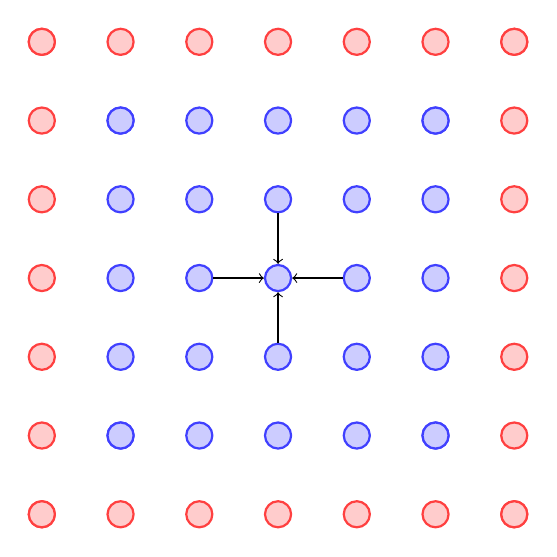
\begin{tikzpicture}
\tikzstyle{place}=[circle,thick,draw=blue!75,fill=blue!20,minimum size=2mm]

\node[place] (p1) at (0,0) {};
\node[place] (p2) at (0,1) {};
\node[place] (p3) at (1,0) {};
\node[place] (p4) at (-1,0) {};
\node[place] (p5) at (0,-1) {};

\node[place] () at (-1,-1) {};
\node[place] () at (-1,1) {};
\node[place] () at (1,-1) {};
\node[place] () at (1,1) {};

\foreach \x in {-2,...,2}
{
  \node[place] () at (\x,2) {};
  \node[place] () at (\x,-2) {};
  \node[place] () at (2,\x) {};
  \node[place] () at (-2,\x) {};
}

\draw[->] (p2) to (p1);
\draw[->] (p3) to (p1);
\draw[->] (p4) to (p1);
\draw[->] (p5) to (p1);

\tikzstyle{place}=[circle,thick,draw=red!75,fill=red!20,minimum size=2mm]

\foreach \x in {-3,...,3}
{
  \node[place] () at (\x,3) {};
  \node[place] () at (\x,-3) {};
  \node[place] () at (3,\x) {};
  \node[place] () at (-3,\x) {};
}



\end{tikzpicture}
}
\end{figure}

Si l'on suppose que la mise à jour de la grille par application du stencil n'est pas calculée en place --- c'est-à-dire que l'on dispose d'un tableau d'entrée dans lequel les éléments sont seulement lus, et d'un tableau de sortie où les résultats du calcul du stencil sur chaque élément sont stockés --- le stencil peut être appliqué à chaque élément bleu en même temps. Le parallélisme se trouve donc de manière très aisée dans ce type de problème. Avec une  machine possédant autant de cœurs que d'éléments dans la grille, la mise à jour de la grille se fait donc en une seule étape et tous les processeurs exécutent les mêmes instructions, simplement sur des éléments différents ; le calcul est donc bien adapté à une carte graphique qui regroupe justement ces caractéristiques : nombre élevé de cœurs et un même code s'exécutant sur tous ceux-ci. Puisque le calcul n'est pas en place, pour l'appliquer plusieurs fois d'affilée il suffit d'intervertir les grilles d'entrées et de sortir entre chaque mise à jour, ou bien de recopier la sortie vers l'entrée, ce qui est toutefois plus lent. Par ailleurs le parallélisme peut s'obtenir grâce aux capacités vectorielles des processeurs : par exemple pour la mise à jour des éléments de toute une ligne en même temps sur l'exemple précédent, il suffit de faire quatre additions vectorielles : la ligne est sommée avec celle du dessus, celle du dessous, elle-même décalée d'un élément vers la gauche, elle-même décalée d'un élément vers la droite. Il y a donc possibilité de parallélisme à plusieurs niveaux du matériel : intraprocesseur et interprocesseur.

Le parallélisme s'obtient presqu'immédiatement pour les stencils, mais cela ne signifie pas pour autant qu'il est efficace. En effet les problèmes qui les utilisent, nécessitent généralement beaucoup de mémoire (qui est de plus doublée en considérant que les calculs ne sont pas en place), ce qui rend l'efficacité moindre. La mémoire des ordinateurs est hiérarchique et les lectures/écritures rapides des éléments d'une grille ne peuvent se faire que sur de petites parties proches des processeurs. Il s'agit de la mémoire \emph{cache} --- ou plus simplement, du cache --- qui est elle-même hiérarchique. Les plus grandes difficultés dans la parallélisation des stencils sont ainsi liées à la bonne utilisation de la mémoire, afin d'éviter les chargements/déchargements inutiles de données\footnote{Notons par ailleurs que l'amélioration des performances par du recouvrement calculs/communications n'a pas été abordée lors du stage.}. En effet si nous supposons que chaque cœur est associé à un élément de la grille et en considérant de nouveau le cas de la figure \ref{fig:stencil_base}, chaque élément nécessite les valeurs des quatre éléments autour de lui pour effectuer le calcul. Si chaque cœur chargeait séparément ces valeurs, il faudrait donc l'équivalent de cinq grilles en mémoire (quatre --- identiques --- pour les valeurs de départ et une pour le résultat), alors qu'en réalité seule deux sont nécessaires. La difficulté de la parallélisation des stencils réside donc dans la façon d'utiliser la mémoire, notamment en faisant en sorte que les cœurs soient disposés comme les éléments de la grille et partagent avec leurs voisins les éléments qu'ils utilisent, afin d'une part de maximiser la réutilisation des données, et d'autre part de minimiser les temps de transfert.

\subsection{Organisation de la mémoire matérielle}

L'élément premier de la hiérarchie de la mémoire est le disque dur, qui est suivi par la mémoire RAM plus rapide mais plus petite. Nous supposons ici que le problème peut toujours être contenu en mémoire RAM. En-dessous d'elle se situe la mémoire des processeurs, le cache, qui limite les performances car elle ne peut pas contenir les données du problème entier. Le cache est lui-même décomposé en plusieurs niveaux qui sont de plus en plus petits et rapides (de la RAM vers les cœurs), mais de moins en moins partagés par les cœurs. La figure \ref{fig:memoire_base} donne un exemple de cette hiérarchie pour deux processeurs et une carte graphique. Les caches des processeurs possèdent trois niveaux dont les deux premiers sont exclusifs tandis que le dernier (noté L3) est partagé de manière directe entre les cœurs d'un même processeurs, il est également interconnecté entre tous les cœurs mais avec un accès \emph{non-uniforme}. Chaque processeur central est alors appelé un nœud ou un banc NUMA et l'accès au cache L3 d'un autre banc est plus coûteux que l'accès au sien. Quant au processeur graphique il possède une mémoire globale assez grande, et des petites mémoires partagées entre des groupes --- ou \emph{warps} --- de $16$ ou $32$ cœurs. Cette mémoire n'est pas un cache pour le processeur graphique, car celui-ci n'opère pas de cohérence des données entre les cœurs : c'est au programmeur de savoir quel cœur possède la donnée la plus à jour. Il en résulte une plus grande complexité dans la gestion de la mémoire graphique, et notamment l'obligation d'avoir de temps en temps des synchronisations entre les cœurs d'un même warp. 

\begin{figure}[!h]
  \caption{Exemple de structure hiérarchique de la mémoire (en vert) d'un ordinateur possédant deux processeurs et une carte graphique (les cœurs de calcul sont en rouge).}
  \label{fig:memoire_base}
  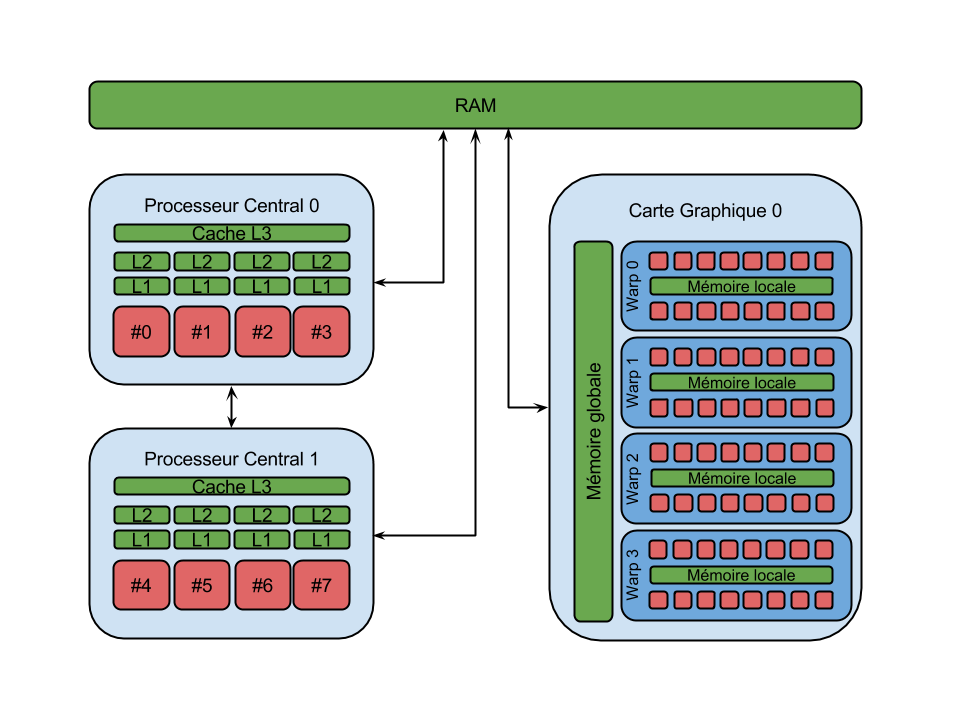
\includegraphics[width=\textwidth]{Memory.png}
\end{figure}

La hiérarchie de la mémoire va limiter certaines optimisations du parallélisme (car la quantité de données utilisable par les calculs parallèles est alors réduite), et il convient d'écrire les programmes en adéquation avec les capacités du matériel (ce point sera évoqué dans la seconde partie de la section \ref{sec:desc_mat_tests}). Des problèmes similaires interviennent avec les processeurs graphiques qui peuvent effectuer beaucoup plus d'opérations à la seconde que les processeurs centraux, mais nécessitent des chargements de données de la RAM vers leur mémoire qui sont plus coûteux en temps qu'entre la RAM et les caches d'un processeur central.

La section suivante précise les objectifs d'un DSEL dédié aux stencils, du côté sémantique comme du côté des performances en présentant notamment une technique de parallélisation adaptée à la hiérarchie de la mémoire (cf section \ref{sec:obj_perf}).

\section{Conception d'un DSEL pour les stencils}

Principalement deux DSEL existent déjà pour les stencils : \textsf{Pochoir} et \textsf{Blitz++}. Cependant les deux souffrent de plusieurs désavantages que nous avons essayé d'éviter dans le DSEL élaboré pendant le stage. Les deux nécessitent par exemple l'apprentissage de plusieurs mots-clés qui fonctionnent généralement comme des balises HTML : ils ouvrent des sections spécifiques puis les ferment. Cela facilite certainement l'analyse du code par le compilateur dans le cas de \textsf{Pochoir}, mais dans les deux cas cela est contraire au paradigme assez répandu de l'utilisation de fonctions à arguments (ou bien méthodes) pour initialiser ou faire des calculs sur des éléments (objets, structures, etc\ldots) --- que ce soit dans la programmation orientée objet, impérative ou fonctionnelle. Par ailleurs \textsf{Blitz++} souffre de l'utilisation de \emph{macros}, des parties de codes qui sont rajoutées dans le code par le compilateur avant la compilation, mais sont parfois présentées comme des fonctions au développeur ; en cas d'erreur lors de la compilation il peut donc il y avoir confusion sur son origine. Enfin les deux DSEL se focalisent sur une exécution sur CPU uniquement, alors que les GPU sont très adaptés à ce genre d'opérations.

En dehors des DSEL, un autre moyen d'aider le développeur est de le laisser écrire le code tel que d'habitude et de modifier le compilateur afin de détecter automatiquement les stencils. Compte-tenu de la complexité des codes actuels et des compilateurs cela nécessite un travail trop important pour le cadre du stage. Il aurait aussi été possible de développer un langage dédié au problème --- dénommé DSL (pour \emph{Domain Specific Language}, équivalent de \emph{langage dédié à un domaine}) ---, mais cela n'est pas avantageux à plusieurs titres. D'une part il est alors nécessaire de créer un compilateur associé. D'autre part un langage dédié au problème ne permet par définition pas d'en traiter d'autres, or les stencils ne sont la plupart du temps qu'une étape dans la résolution d'un problème plus élaboré. Un langage dédié aurait donc du être interfacé avec d'autres. Au contraire un DSEL est développé dans un langage préexistant, et utilisable directement dans ce langage. Le programmeur peut alors utiliser plusieurs DSEL dans le même code, et résoudre des problèmes complexes avec un formalisme adapté à chacun d'entre eux (et par là-même avoir de meilleures performances). Le DSEL est ainsi une solution intermédiaire efficace, qui nous a semblé adaptée à l'objectif du stage qui est la parallélisation automatique d'une catégorie spécifique de programmes. Il se situe dans la même classe de bibliothèques que \textsf{Blitz++} ou les \textsf{BLAS} et en reprend certains concepts.

Todd L. Veldhuizen, le concepteur de \textsf{Blitz++}, a introduit la notion d'\emph{active libraries} (\emph{bibliothèques actives}) \cite{Art20} afin de décrire ce qu'un DSEL notamment (ainsi que le compilateur associé) doit proposer a minima. Ces bibliothèques doivent tirer partie de toutes les possibilités dont elles disposent : à la fois la sémantique de l'expression qui est codée par le biais du DSEL, et les performances offertes par des bibliothèques spécialisées dans certains types d'opérations. Elles sont actives car elles ne fournissent pas seulement des méthodes optimisées, elles les choisissent en fonction de l'expression. Par ailleurs Todd Veldhuizen propose dans l'article \cite{Art22} trois aspects à développer dans le DSEL afin d'obtenir des performances : \emph{Pretty, Safe, Fast} (pour élégant, sûr, et rapide). Ces trois aspects sont au centre des préoccupations avec lesquelles le DSEL a été développé au cours du stage. Tandis que nous regroupons les caractères élégant et sûr dans les objectifs sémantiques, la rapidité est quant à elle liée à la performance.

\subsection{Objectifs sémantiques}
\label{sec:obj_sem}

Le premier objectif sémantique est de pouvoir décrire toutes les formes de stencils. Le stencil lui-même est déterminé par les indices des éléments qui rentrent en jeu dans le calcul. Dans l'exemple précédent de stencil à quatre points dans une grille en deux dimensions, si nous considérons comme origine du repère un élément quelconque à mettre à jour alors les éléments nécessaires à sa mise à jour ont pour indices $(-1,0)$, $(1,0)$, $(0,-1)$ et $(0,1)$. La simple connaissance de ces indices relatifs permet de retrouver le motif du stencil, il est donc primordial de pouvoir déclarer simplement les indices entrant en jeu dans le stencil. Dans la suite du document nous appelons ces indices relatifs les \emph{indices de décalage}.

Par ailleurs un stencil peut nécessiter des coefficients. Par exemple dans le cas de l'algorithme classique Jacobi, ces coefficients sont constants et ne sont liés qu'aux positions relatives des éléments accédés par le stencil. Si la grille des éléments est stockée dans un tableau $A$ à deux dimensions, l'équation associée à la mise à jour d'un élément d'indice global $(i,j)$ par le stencil pourrait donc s'écrire de façon mathématique comme l'équation \ref{eq:st0_fxd} où les $c_x$ sont les coefficients fixes.
\begin{equation}
\label{eq:st0_fxd}
A[i,j] = c_1 \times A[i-1,j+0] + c_2 \times A[i+1,j+0] + c_3 \times A[i+0,j-1] + c_4 \times A[i+0,j+1]
\end{equation}
Les coefficients étant dans ce cas liés aux indices de décalage, un DSEL doit donc permettre la possibilité de déclarer les deux en même temps.

Toutefois cet exemple ne regroupe pas tous les cas imaginables, il est également possible d'abstraire l'opération de réduction qu'est ici la somme, de même que l'opération liant les coefficients aux éléments de la grille (notamment si les éléments ne sont pas de simples scalaires, mais des matrices ou des nombres complexes). Nous notons respectivement ces deux opérations $\oplus$ et $\otimes$. L'équation \ref{eq:st0_fxd} se réécrit alors en l'équation \ref{eq:st1_fxd}.
\begin{equation}
\label{eq:st1_fxd}
A[i,j] = c_1 \otimes A[i-1,j+0] \oplus c_2 \otimes A[i+1,j+0] \oplus c_3 \otimes A[i+0,j-1] \oplus c_4 \otimes A[i+0,j+1]
\end{equation}
La nature des opérateurs doit donc apparaître dans la définition du stencil.

Une autre variante sur les coefficients consiste à les considérer variables en fonction non seulement de l'élément calculé, mais aussi en fonction du décalage pour chaque élément entrant en compte. Une telle possibilité est parfois utile, notamment dans les calculs de chromodynamique quantique. Nous notons $f$ la fonction qui renvoie le coefficient en fonction des différents indices (celui de l'élément traité, et celui des éléments utilisés). En deux dimensions $f$ prend donc quatre arguments et l'équation \ref{eq:st1_fxd} devient l'équation \ref{eq:st1_var}.
\begin{equation}
\label{eq:st1_var}
\begin{aligned}
A[i,j] = & f(i, j, -1,  0) \otimes A[i-1,j+0] \oplus \\
         & f(i, j,  1,  0) \otimes A[i+1,j+0] \oplus \\
         & f(i, j,  0, -1) \otimes A[i+0,j-1] \oplus \\ 
         & f(i, j,  0,  1) \otimes A[i+0,j+1]
\end{aligned}
\end{equation}

Cette dernière équation est un peu plus complexe à abstraire car les coefficients ne sont plus seulement liés aux indices relatifs de décalage. En effet le stencil est alors défini par une fonction supplémentaire, et la déclaration d'une telle fonction peut-être laborieuse. Pour rendre cette fonction plus simple à déclarer, $f$ devient alors une fonction d'accès uniquement qui au lieu de déterminer la valeur du coefficient grâce au paramètre, permet d'accéder à l'endroit où se situe le coefficient pré-calculé dans un tableau. La déclaration de $f$ est alors plus aisée, mais le stencil nécessite également la connaissance du tableau de coefficients (que l'utilisateur doit lui-même pré-remplir). $f$ prend alors un cinquième argument (le tableau) noté $C$.

Ce choix d'avoir un tableau supplémentaire, permet en outre d'abstraire la structure des données, et il serait souhaitable de l'utiliser non seulement pour les coefficients variables, mais aussi pour les éléments de la grille de calcul. Cette fonction $g$ prend alors en argument l'indice --- non-relatif, global --- de l'élément courant ainsi que le tableau de la grille. De cette façon la grille peut être stockée sous une forme entièrement paramétrable : \emph{row major}\footnote{Dans le cas d'une grille à deux dimensions, la disposition \emph{row major} consiste à placer les lignes les unes à la suite des autres dans un tableau à une dimension.}, \emph{column major}\footnote{Idem note précédente, par colonne.} ou autre. On peut alors réécrire la dernière équation, en considérant maintenant le fait que le calcul ne se fait pas en place et que le résultat est stocké dans un tableau $B$, et l'on obtient l'équation \ref{eq:st2_var}.
\begin{equation}
\label{eq:st2_var}
\begin{aligned}
g(i,j,B) = & f(i, j, -1, \quad 0, C) \otimes g(i-1, j+0, A) \, \oplus \\
           & f(i, j, \quad 1, \quad 0, C) \otimes g(i+1,j+0, A) \, \oplus \\
           & f(i, j, \quad 0, -1, C) \otimes g(i+0,j-1, A) \, \oplus \\ 
           & f(i, j, \quad 0, \quad 1, C) \otimes g(i+0,j+1, A)
\end{aligned}
\end{equation}

En résumé l'application d'un stencil sur une grille nécessite l'enregistrement dans le DSEL des éléments suivants : 
\begin{itemize}
\item les indices de décalage (avec éventuellement les coefficients constants) ;
\item la fonction d'accès aux coefficients variables et le tableau associé (s'il n'y a pas de coefficients constants) ;
\item les opérateurs de réduction $\oplus$ et d'application du coefficient à l'élément $\otimes$ ;
\item les tableaux d'entrées et sorties ;
\item la fonction d'accès pour ces deux tableaux.
\end{itemize}

Éventuellement, le DSEL peut prévoir plusieurs types d'agrégations :
\begin{itemize}
\item la combinaison de plusieurs motifs de stencils en un seul ;
\item la possibilité d'appliquer le même motif sur plusieurs tableaux à la fois ;
\item le \emph{stream} (ou \emph{flux}) de plusieurs stencils à la suite sur un unique tableau de départ, les tableaux intermédiaires étant alors omis.
\end{itemize}

Les caractères élégant et sûr du DSEL sont nécessairement dépendants du langage choisi. En ce qui concerne l'élégance, il s'agit d'utiliser le moins de symboles et fonctions possibles, et de cacher tous les paramètres calculables automatiquement. Pour la sûreté le but est de détecter certains types d'erreurs comme l'utilisation du même tableau en entrée et en sortie (en supposant que le calcul en place n'a pas lieu d'être) et l'usage d'indices de décalage en dehors de la grille.

\subsection{Objectifs de performances}
\label{sec:obj_perf}

Les performances peuvent s'obtenir grâce à l'adaptation du code tant par rapport au matériel que par rapport aux algorithmes de calculs utilisés. Deux voies complémentaires doivent être explorées : la réutilisation maximale des données dans le cache (qui induit le principe de \emph{tuilage}), le calcul du plus grand nombre de paramètres possibles lors de la compilation (les paramètres en jeu étant alors \emph{statiques}).

\subsubsection*{Tuilage de stencil} 

Avant de déterminer quels paramètres peuvent être calculés à la compilation, il est nécessaire de voir plus en détail comment la parallélisation va être effectuée au sein du stencil. Puisque les tableaux utilisés dans les calculs sont généralement trop grands pour la mémoire respectivement cache ou locale proche des processeurs respectivement centraux ou graphiques, la grille de l'exemple précédent est divisée en blocs que nous appelons \emph{macro-tuiles}. La taille de chaque macro-tuile est choisie de façon que la mémoire utilisée par les calculs tienne soit dans les caches L3 soit dans la mémoire locale (cf figure \ref{fig:memoire_base}). La façon de paralléliser la macro-tuile est la suivante : chaque processeur central (ou warp dans le cas des cartes graphiques) est lié à une macro-tuile et chaque cœur va appliquer le stencil sur un ou plusieurs éléments différents\footnote{La notion de \emph{tuile} sera utilisée dans la section \ref{sec:desc_mat_tests} et fait référence à la parallélisation au sein d'un cœur, et non au sein d'un processeur.}. Si l'on reprend l'exemple de la figure \ref{fig:memoire_base} avec le stencil à $4$ points, la parallélisation par tuilage sur la carte graphique sur une grille de $10$ par $10$ éléments va pouvoir se faire en la découpant en quatre blocs carrés chacun associé à un warp. Chaque \emph{warp} possédant chacun $16$ cœurs va appliquer le stencil sur une macro-tuile de dimensions $4 \times 4$. La figure \ref{fig:stencil_mtile} représente cette situation en précisant par des bordures en pointillé les éléments fantômes que le \emph{warp} $0$ coloré en jaune devra contenir. Bien que les seuls fantômes à la base soient les éléments rouges en bordure de la grille, chaque \emph{warp} a besoin de charger les éléments autour de lui compte-tenu de la forme du stencil.

\begin{figure}[!h]
\floatbox[{\capbeside\thisfloatsetup{capbesideposition={right,center},capbesidewidth=4cm}}]{figure}[\FBwidth]
{\caption{Exemple de tuilage d'une grille en deux dimensions sur une carte graphique possédant $4$ \emph{warps}. Les éléments calculés sont de couleur bleu, et les éléments fantômes en rouge ainsi que dans les cadres en pointillé pour ce qui concerne le \emph{warp} $0$.}\label{fig:stencil_mtile}}
{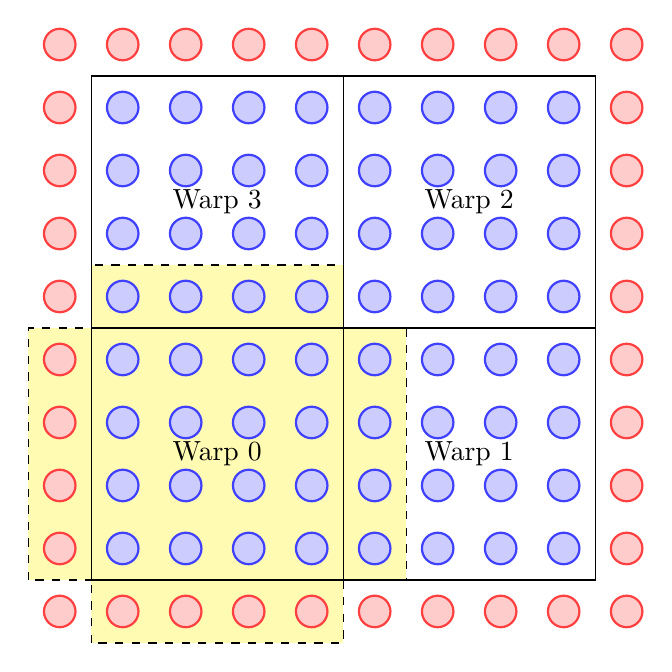
\begin{tikzpicture}[scale=0.8]
\tikzstyle{place}=[circle,thick,draw=blue!75,fill=blue!20,minimum size=4mm]

\draw[dashed,fill=yellow!30] (0.5,-0.5) rectangle (4.5,0.5);
\draw[dashed,fill=yellow!30] (-0.5,0.5) rectangle (0.5,4.5);
\draw[dashed,fill=yellow!30] (0.5,4.5) rectangle (4.5,5.5);
\draw[dashed,fill=yellow!30] (4.5,0.5) rectangle (5.5,4.5);

\draw[fill=yellow!30] (0.5,0.5) rectangle (4.5,4.5);
\draw (4.5,4.5) rectangle (8.5,8.5);
\draw (0.5,4.5) rectangle (4.5,8.5);
\draw (4.5,0.5) rectangle (8.5,4.5);


\foreach \x in {1,...,8}
{
  \foreach \y in {1,...,8}
  {
    \node[place] () at (\x,\y) {};
  }
}

\node () at (2.5,2.5) {Warp 0};
\node () at (6.5,2.5) {Warp 1};
\node () at (6.5,6.5) {Warp 2};
\node () at (2.5,6.5) {Warp 3};


\tikzstyle{place}=[circle,thick,draw=red!75,fill=red!20,minimum size=4mm]

\foreach \x in {0,...,9}
{
  \node[place] () at (\x,0) {};
  \node[place] () at (\x,9) {};
}
\foreach \y in {1,...,8}
{
  \node[place] () at (0,\y) {};
  \node[place] () at (9,\y) {};
}



\end{tikzpicture}
}
\end{figure}

L'intérêt du tuilage est de pouvoir faire rentrer tous les éléments nécessaires à la mise-à-jour d'une macro-tuile dans le cache L3 (ou la mémoire locale) du processeur (ou du warp) qui la traite. De plus nous ne perdons pas en parallélisation (dans l'exemple précédent tous les éléments sont calculés en même temps puisqu'il y a autant d'éléments que de cœurs). La gestion de la mémoire n'est cependant pas parfaite, puisque chaque macro-tuile nécessite sa zone fantôme dont les éléments ne seront utilisés qu'une seule fois. D'autres formes de découpage que les blocs carrés sont possibles, notamment dans le cas de stencils asymétriques (qui nécessitent plus de voisins dans une direction que dans l'autre) où des rectangles sont adaptés, toutefois cette problématique n'a pas été étudiée dans le cadre de ce stage. Par ailleurs si le stencil devait être appliqué en place, notons qu'une synchronisation des cœurs est alors nécessaire suivie par le rechargement de toutes les zones fantômes depuis les macro-tuiles voisines, ce qui est coûteux en temps. Une solution alternative fondée sur des calculs redondants (supposés moins coûteux) est présentée dans le cadre des améliorations possibles, à la section \ref{sec:amelior_backend}.

Le cas de la figure \ref{fig:stencil_mtile} est simple car il y a autant de cœurs que d'éléments à calculer ; il reste donc à gérer le cas général où la grille de base est beaucoup plus grande que le nombre de cœurs, et dont les dimensions n'en sont pas forcément des multiples entiers. En pratique les macro-tuiles vont alors être calculées les unes après les autres. Et si la taille de la grille n'est pas multiple du nombre de processeurs dans chacune des dimensions, une macro-tuile sera ajoutée et ses éléments dépassant de la grille ne seront pas calculés. 

De même cet exemple est uniquement en deux dimensions, mais certains calculs nécessitent des stencils sur des grilles à quatre dimensions, notamment en chromodynamique quantique. Certains articles \cite{Art1,Art11} développent des techniques spécifiques pour y remédier, tout en gardant une certaine réutilisation des données. Ces techniques sont très spécialisées et ne seront pas évoquées ici, toutefois il convient de savoir qu'elles existent et que le DSEL devrait être capable à terme de les intégrer.

\subsubsection*{Paramètres statiques}

Les paramètres statiques vont permettre d'éviter au programme certains calculs lors de l'exécution (qui sont tout de même faits lors de la compilation), et d'être donc légèrement plus rapide. Les principaux paramètres entrant en jeu pour la parallélisation sont :
\begin{itemize}
\item le nombre de dimensions de la grille ;
\item le nombre d'éléments dans chaque dimension de la grille ;
\item le nombre d'éléments du stencil ;
\item les indices de décalage du stencil ;
\item la taille des zones fantômes de la grille ;
\item la quantité de mémoire disponible en mémoire cache de niveau 3 ou en mémoire locale ;
\item le nombre de processeurs et cœurs disponibles à l'intérieur ;
\item la forme et la taille des macro-tuiles ;
\item la taille des zones fantômes des macro-tuiles.
\end{itemize}

Tous ces paramètres peuvent (et doivent) être statiques, hormis le nombre d'éléments de la grille qui par choix est déterminé à l'exécution. En effet nous supposons que le programme doit être compilé pour chaque problème différent (donc avec des stencils différents) mais pas pour chaque instance du même problème, où seul le nombre d'éléments (donc la précision de la résolution) change. C'est cette approche qui est aussi utilisée dans \textsf{QIRAL}. Le problème est alors de savoir comment calculer ces paramètres statiquement --- certaines peuvent se déduire les unes des autres ---, et cela dépend du langage choisi pour le DSEL, notamment si le langage autorise la méta-programmation, une façon de modifier le comportement de certaines fonctions à la compilation. Le calcul de la taille des macro-tuiles et de leur zone fantôme est détaillé dans la section \ref{sec:param_tuile} du chapitre suivant.

Plus généralement, d'autres paramètres aidant dans l'ordonnancement des calculs (ainsi que des transferts de mémoire, notamment si plusieurs types de processeurs sont disponibles) pourraient (mais difficilement) être déterminés lors de la compilation ; cela n'a pas été étudié dans le cadre du stage. Au reste la tendance actuelle est justement à l'opposé : c'est le rôle des supports d'exécutions que de gérer l'ordonnancement lors de l'exécution. 


Les objectifs du DSEL à implanter sont donc de plusieurs natures : à la fois centrés sur la sémantique et toutes les informations nécessaires à un calcul de stencil, et aussi sur les performances de ce calcul. Le travail d'implantation concerne donc tout autant l'interface utilisateur mise en place que la façon de paralléliser les calculs. Par ailleurs réimplanter les mécanismes permettant la parallélisation sur les machines modernes est une tâche bien trop lourde qu'il n'est pas possible de réaliser nous-mêmes, ce pour quoi nous utilisons une bibliothèque tierce qui lance elle-même les calculs optimisés par le DSEL. Cette bibliothèque, l'interface et l'implantation des objectifs sont détaillés dans le chapitre suivant.
